\documentclass{standalone}

\usepackage{tikz}

\usetikzlibrary{positioning, chains, shapes.geometric, fit, shapes, arrows.meta, calc, backgrounds}

\begin{document}

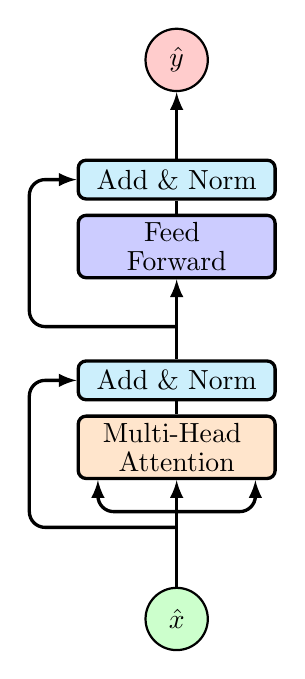
\begin{tikzpicture}[
    >=LaTeX, % Use default LaTeX arrows
    very thick,
    arrow/.style={
        -latex,
        very thick,
        rounded corners=0.2cm
    },
    block/.style={
        rectangle,
        fill=gray!10,
        rounded corners=3mm,
        draw,
        very thick
    },
    add_norm/.style={
        rectangle,
        fill=cyan!20,
        rounded corners=1mm,
        inner xsep=0em,
        inner ysep=0.25em,
        minimum height=1.4em,
        align=center,
        text width=2.5cm,
        draw,
        very thick
    },
    mha/.style={
        rectangle,
        fill=orange!20,
        rounded corners=1mm,
        inner xsep=0em,
        inner ysep=0.25em,
        minimum height=1.4em,
        align=center,
        text width=2.5cm,
        draw,
        very thick
    },
    linear_layer/.style={
        rectangle,
        fill=blue!20,
        rounded corners=1mm,
        inner xsep=0em,
        inner ysep=0.25em,
        minimum height=1.4em,
        align=center,
        text width=2.5cm,
        draw,
        very thick
    },
    input/.style={ % Input or output node
        circle,
        minimum width=2.25em,
        draw,
        fill=green!20,
        thick
    },
    output/.style={ % Input or output node
        circle,
        minimum width=2.25em,
        draw,
        fill=red!20,
        thick
    }
]

    \node[input] (iemb) at (1.25,0.4) {$\hat{x}$};


    % Encoder, 1st layer
    \node[add_norm] (add1) at (1.25,3.43) {Add \& Norm};
    \node[mha] (attn1) at (1.25,2.58) {Multi-Head \vspace{-0.05cm} \linebreak Attention};
    \draw[] (attn1) -- (add1);
    % Encoder 2nd sub-layer
    \node[add_norm] (add4) at (1.25,5.98) {Add \& Norm};
    \node[linear_layer] (ff1) at (1.25,5.13) {Feed \vspace{-0.05cm} \linebreak Forward};
    \draw[] (ff1) -- (add4);


    \draw[arrow] (add1) -- (ff1);
    \draw[arrow] (iemb) -- (attn1);


    \draw[arrow] (ff1.south)++(0, -0.6) -| ($(add4.west) + (-0.6,-0.5)$) |- (add4.west);
    \draw[arrow] (attn1.south)++(0, -0.6) -| ($(add1.west) + (-0.6,-0.5)$) |- (add1.west);


    \draw[arrow] (attn1.south)++(0, -0.4) -| ($(attn1.south) + (-1,0)$);
    \draw[arrow] (attn1.south)++(0, -0.4) -| ($(attn1.south) + (1,0)$);

    \node[output] (out) at (1.25,7.5) {${\hat y}$};
    \draw[arrow] (add4) -- (out);

\end{tikzpicture}

\end{document}